% -*- Mode:TeX -*-
% LaTeX template for CinC papers                   v 1.1a 22 August 2010
%
% To use this template successfully, you must have downloaded and unpacked:
%       http://www.cinc.org/authors_kit/papers/latex.tar.gz
% or the same package in zip format:
%       http://www.cinc.org/authors_kit/papers/latex.zip
% See the README included in this package for instructions.
%
% If you have questions, comments or suggestions about this file, please
% send me a note!  George Moody (george@mit.edu)
%
\documentclass[twocolumn]{cinc}
\usepackage{graphicx}
\begin{document}
\bibliographystyle{cinc}

\title{Dynamic Time Warping with Gradient Boosting Tree Ensemble for \\
12-Lead Electrocardiogram Multilabel Classification}

\author {Alexander W Wong$^{1}$, Weijie Sun$^{2}$, Sunil V Kalmady$^{2}$, Padma Kaul$^{2}$, Abram Hindle$^{1}$\\
\ \\
 $^1$ University of Alberta, Edmonton, Canada \\
$^2$ Canadian VIGOUR Center, Edmonton, Canada }

\maketitle

\begin{abstract}

Standard 12-lead electrocardiograms (ECGs) are commonly used to detect cardiac irregularities such as atrial fibrillation, blocks and irregular complexes.
For the Physionet/CinC 2020 Challenge, we built an algorithm using gradient boosted tree ensembles fitted on morphology and signal processing features.

We used the ecgpuwave implementation of the Pan Tompkins method to detect the P-wave, QRS complex, and T-wave.
We selected templates that exhibited maximum similarity with the rest of the ECG records in the same class using minimum distance criteria to isolate candidate templates for each cardiac abnormality.
We leveraged these templates using Dynamic Time Warping (DTW), an algorithm used for measuring similarity between temporal sequences of varying speeds.
From the annotated signals we derived morphology related durations, amplitudes, and intervals.
Additional signal representation techniques, including discrete Fourier transformations and polynomial function fitting, were also used to extract features.

We concatenate the features for all 12 leads and fit an ensemble of gradient boosting trees to predict probabilities of ECG instances belonging to each class.
We evaluated using a 5-fold cross validation split of the provided dataset.

\end{abstract}

\section{Introduction}

Cardiovascular diseases are a non-communicable leading cause of death, responsible for an estimated 17.8 million fatalities world wide in 2017~\cite{roth_global_2018}.
The electrocardiogram (ECG) is the most effective tool and current best practice strategy for detecting cardiac diseases, outperforming screening history and physical examinations in accuracy and sensitivity~\cite{harmon_effectiveness_2015}.
However, ECG interpretation is a complex and highly skilled task undertaken by multiple health care professionals ranging from physicians, nurses, paramedics, and technicians.
Multiple studies have been conducted highlighting disagreements between non-cardiologists and cardiologist reference ECG interpretations, with up to a 33\% interpretation error rate~\cite{mele_improving_2008}.
Despite active research in computerized interpretations of ECGs, trained human over-reading and confirmation is required and emphasized in published reports~\cite{schlapfer_computer-interpreted_2017}.

This work classifies standard 12-lead ECGs to their clinical diagnosis as part of the PhysioNet/Computing in Cardiology Challenge~\cite{physionet_challenge_2020}.
We developed a multi-label classification algorithm using natural language and signal processing inspired features and a gradient boosting tree ensemble.

\subsection{Print font}

Please use Times New Roman font. Use of this font by all authors ensures
that our papers are produced consistently with a professional appearance.


 \subsection{ Print size}  

Follow the information given in Table 1 for all font print sizes and styles.

\section{Title block}
 
On the first page, the title, authors, and institution(s) should be
positioned and aligned as above.

\subsection{Title} 
 
Do not use abbreviations in the title and keep to one or two
lines. Remember that the title should be easily understood when cited as a
reference in another publication. Make sure the title is centered. Note the
use of capital letters, as shown in the example above. Do not place a
period at the end of the title.

\subsection{ Author line}  
 
If it is essential to link authors to different institutions, use a small
superscript at the end of each family name and link to each institution. No author degrees should be
included. No periods should appear in the author line.

 \subsection{ Institution address} 

 This address identifies the institution(s). It is not a postal address and
 should not contain postal or zip codes. A full postal address is given at
 the end of the paper under `Address for correspondence'. Do not put line
 spaces between address lines or use a period at the end.
 
 \section{ Tables and figures}
\subsection{Tables} 
\vspace{-4 mm}
\begin{table}[htbp]
\caption{\label{tab:font} Print sizes for different parts of the paper.}
\vspace{4 mm}
\centerline{\begin{tabular}{lcr} \hline\hline
Text    & Point size    & Type \\ \hline
Title   & 14 point      & Bold \\
Author line     & 12 point      & \\
Institution line        & 12 point      & \\
Abstract heading        & 11 point      & Bold \\
All other headings      & 12 point      & Bold \\
Abstract text   & 10 point      & Italic \\
References and address  & 9 point       & \\
All other text  & 10 point      & \\ \hline\hline
\end{tabular}}

\end{table}

Keep \ the layout of \ tables simple. Avoid  heavy lines and boxes.

\subsection{ Figures}   

Figures can fit across both columns if necessary. Include all figures, with
captions, in the text document at their desired locations, i.e., not at the
end. To make sure that all labels are legible, use at least 9-point
font. Use a line thickness of at least 0.5 mm in the body of the figure.

\begin{figure}[h]
%\centering
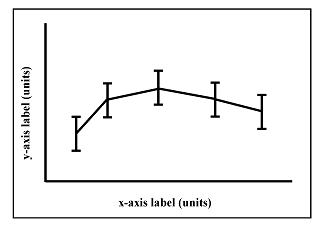
\includegraphics[width=7.9cm]{fig/graph.png}
\caption{Put the figure legend here, at the bottom, clearly describing the
  figure.}
\label{FIGURA1}
\end{figure}

Leave a line space after a figure legend. Be cautious with background
colors in figures because they can make printed figures hard to read.

\section{Final page}

The text on the final page should be arranged so that both columns are
approximately the same length.

\balance

\section{Style of references}     

All references should be included in the text in square brackets in their
order of appearance, e.g., \cite{tag}, \cite{tag,ito}, or
\cite{tag,ito,fardel,buncombe}. In the reference list, use the Vancouver
style (see IEEE Transactions on Biomedical Engineering or Annals of
Biomedical Engineering). The main goal is to be consistent in your
formatting of references.

References to \emph{Computers in Cardiology} (or \emph{Computing in
  Cardiology}) proceedings should include the volume and page numbers,
unless no page numbers were included (post-2016). Check the style in the
examples below.


\section{ Final checks }     
 
Print this template without resizing or centering and compare with your
final paper to ensure that you have not accidentally changed margins and
layout.


\section*{Acknowledgments}
We would like to thank Eric Ly and Leiah Luoma for their help and guidance during our research journey.

\bibliography{main}

\begin{correspondence}
Alexander W. Wong\\
Department of Computing Science\\
2-32 Athabasca Hall\\
University of Alberta\\
Edmonton, Alberta, Canada\\
T6G 2E8\\
alex.wong@ualberta.ca
\end{correspondence}

\end{document}

